
\input{../Common/commands}

\begin{document}

\graphicspath{ {../Common/images/} }
\input{../Common/map}
\graphicspath{ {images/} }

%----------------------------------------------------------------
% MAIN TABLE DEFINITION
% ----------------------------------------------------------------
\newcommand*\maintab[1]{
\setsepchar{ }
\readlist\args{#1}
{\tiny \def\arraystretch{2} \setitemize[0]{leftmargin=0.5em, labelsep=0.2em}
  \begin{tabular}{|P{0.04\textwidth}|P{0.04\textwidth}|P{0.25\textwidth}|P{0.25\textwidth}|P{0.25\textwidth}|}
    \hline
    \multicolumn{2}{|P{0.08\textwidth}|}{\multirow{2}{*}{\parbox[c]{0.11\textwidth}{\bfseries \raggedleft {[S]} statistics {[M]} machine learning}}}&\multicolumn{3}{c|}{\bfseries Type of dependent [S] / target [M] variable}\\
    \cline{3-5}
    \multicolumn{2}{|P{0.08\textwidth}|}{}&\textbf{categorical}&\textbf{numeric}&\textbf{probability of categorical}\\ 
    \hline
    &\rotatebox[origin=c]{90}{\toleft{0.5em}{\bfseries categorical}}&\parbox[c][16.5ex][t]{0.25\textwidth}{\begin{jvklst1}\item\hyperlink{classification-trees}{\HL{\args[1]}{supervised segmentation using impurity measures (can be used for the numeric-categorical combination if numeric attributes converted to categories) [M] }}\end{jvklst1}}&\parbox[c][16.5ex][t]{0.25\textwidth}{\begin{jvklst1}\item\hyperlink{regression-trees}{\HL{\args[2]}{supervised segmentation using variance measures [M]}}\end{jvklst1}}&\parbox[c][16.5ex][t]{0.25\textwidth}{\begin{jvklst1}\item\hyperlink{probability-estimation-trees}{\HL{\args[3]}{probability estimation tree [M]}}\end{jvklst1}}\\ [-2ex] 
&&\makebox[0.26\textwidth][r]{\HL{\args[9]}{\large \cellmarker}}&\makebox[0.26\textwidth][r]{\HL{\args[10]}{\large \cellmarker}}&\makebox[0.26\textwidth][r]{\HL{\args[11]}{\large \cellmarker}}\\
    \cline{2-5}
      \multirow{-5.3}{0.04\textwidth}{\rotatebox[origin=c]{90}{\parbox[c][5ex]{0.24\textwidth}{\bfseries Independent variable [S]/ feature [M] type}}}&\rotatebox[origin=c]{90}{\toleft{0.5em}{\bfseries numeric}}&\parbox[c][11ex][t]{0.25\textwidth}{\begin{jvklst1}\item\hyperlink{linear-classifiers}{\HL{\args[4]}{linear classifiers}} \begin{jvklst2}\item\hyperlink{logistic-regression}{\HL{\args[5]}{logistic regression [S]}}\item\hyperlink{svm}{\HL{\args[6]}{support vector machines [M]}} \end{jvklst2}\item\hyperlink{non-linear-classifiers}{\HL{\args[7]}{non-linear classifiers [M]}} \end{jvklst1}}&\parbox[c][11ex][t]{0.25\textwidth}{\begin{jvklst1}\item\hyperlink{regression}{\HL{\args[8]}{statistical regression (linear and non-linear, simple and multivariate) [S]}}\end{jvklst1}\vspace{0.3em}}& \\[-2ex] 
&&\makebox[0.26\textwidth][r]{\HL{\args[12]}{\large \cellmarker}}&\makebox[0.26\textwidth][r]{\HL{\args[13]}{\large \cellmarker}}&\makebox[0.26\textwidth][r]{\HL{\args[14]}{\large \cellmarker}}\\  
    \hline
\end{tabular}}}

\newcommand*\cornertab[1]{
\begin{tikzpicture}[overlay, remember picture]
\node[anchor=north east, xshift=0\textwidth, yshift=0\textwidth] at (current page.north east)
{\hyperlink{main-table}{\resizebox{0.4\textwidth}{!}{\maintab{#1}}}};
\end{tikzpicture}}


%----------------------------------------------------------------
% PAGE TITLE
% ----------------------------------------------------------------
\pgclrred
\title{\headerpres{Data Analysis: \\ Building Models and Predicting Outcomes}}
\author{\vspace{3cm} Institute of Technology Tallaght}
\date{Department of Computing}
\maketitle
\newpage

% ----------------------------------------------------------------
% PAGE TABLE
% ----------------------------------------------------------------
\headerch{Models}
\hypertargettopofpage{main-table}

\maintab{N N N N N N N N F F F F F F}
\begin{itemize}
\item Models are used for predicting a variable, called
  \begin{itemize}
  \item \emph{dependent variable} in the context of statistics
  \item \emph{target variable} in the context of machine learning
  \end{itemize}
\item They are built using properties of data called
  \begin{itemize}
  \item \emph{independent variables} in the context of statistics
  \item \emph{features} in the context of machine learning
  \end{itemize}
\end{itemize}

\newpage



% ----------------------------------------------------------------
% PAGE NAIVE BAYES
% ----------------------------------------------------------------
\headerch{Na\"ive Bayes}
\begin{itemize}
\item A method for estimating the probabilities of target variable values, based on the assumption of true independence among the attributes of the data
\item Complete independence among all attributes is rarely possible in real data sets but the predictions made by the Na\"ive Bayes family of models are nevertheless very good for practical purposes
\item The Na\"ive Bayes formula for the probability of a data instance belonging to class $C_j$, given a certain combination of attribute values, $X_k$, is:
\cornertab{N N N N N N N N F F H F F H}
  $$ P(C_j|X_k) = \dfrac{P(C_j)\prod_{i=1}^d P(x_{ik}|C_j)}{P(X_k)} $$
where the class $C_j$ is a possible value of the categorical target variable, $X_k$ is the vector of given attribute values (i.e. a data instance, identified as $k$), $d$ is the number of attributes used in the model and $x_{ik}$ is the value of attribute $x_i$ in the vector of given attribute values (i.e. in data instance $k$). $P(C_j)$ is the estimated probability of any data instance in the set belonging to class $C_j$ (i.e. the prior probability of $C_j$). $P(x_{ik}|C_j)$ is the estimated probability of attribute $x_i$ having value $x_{ik}$, given that the class is $C_j$. $P(X_k)$ is the estimated probability of data instance $X_k$ ocurring. The formula assumes independence among the attributes, $x_1$, $x_2$... $x_d$.  
\item The model can be used both with numeric and categorical attributes. Probabilities for categorical attributes can be estimated using counts. For numeric attributes probability densities for a suitable distribution (e.g. normal or Poisson) are used.  
\end{itemize}
\newpage

\begin{tabular}{p{0.3\textwidth}p{0.7\textwidth}}
  \headerss{Example} & \\
  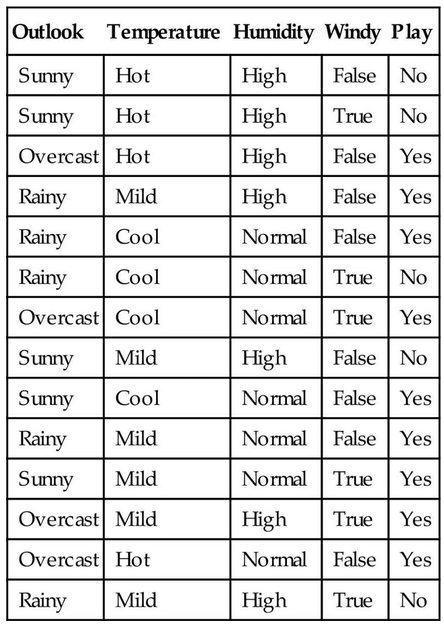
\includegraphics[width=0.3\textwidth]{dm_play_data_table.png} & \begin{minipage}[b]{0.7
      \textwidth}{\tiny First, let's look at the table and see what we can say about whether the game will be played if it is \texttt{\textbf{Sunny}}. There are five instances that have the value of \tb{Sunny} for \texttt{Outlook} and of those 3 are associated with a \tb{No} for \texttt{Play} and 2 with a \tb{Yes}. In terms of probabilities, we can write this as: $$ P(\tb{Yes}|\tb{Sunny}) = \dfrac{2}{5} \quad \quad P(\tb{No}|\tb{Sunny}) = \dfrac{3}{5}$$Based on these values our prediction might be that if it is sunny, the game is more likely not to go ahead than to go ahead. However, we have used only one of the four attributes of the weather availabe to us. It would make more sense to use all data available i.e. all four attributes to make the prediction.
      What if one day the attribute values were: \texttt{Outlook}=\tb{Sunny}, \texttt{Temperature}=\tb{Cool}, \texttt{Humidity}=\tb{High}, \texttt{Windy}=\tb{True} and we wanted to see how likely it was that the game would go ahead? We don't even have a case like that in the table, let alone several cases to use for counting up incidences of \tb{Yes} and \tb{No}. This is where Na\"ive Bayes comes in: 
      \begin{equation}P(\tb{Yes}|\tb{E})=\dfrac{P(\tb{E}|\tb{Yes})P(\tb{Yes})}{P(\tb{E})}\qquad\qquad P(\tb{No}|\tb{E})=\dfrac{P(\tb{E}|\tb{No})P(\tb{No})}{P(\tb{E})}\end{equation}where $\tb{E}$ is used as shorthand for the 'evidence', consisting of the set of values $\{\tb{Sunny},\tb{Cool},\tb{High},\tb{True}\}$, hence $P(\tb{E})=P(\tb{Sunny},\tb{Cool},\tb{High},\tb{True})$.
        
      }\end{minipage} \\ [-0.8em]
  {\fontsize{10}{0}\selectfont \textbf{Source: [DM]}} &   \\ [0.5em]
  
  \multicolumn{2}{p{\textwidth}}{\tiny 
        
  The assumption of independence of attributes allows us to simply multiply the individual probabilities, whether conditional or not:
       $$P(\tb{E}|\tb{Yes})=P(\tb{Sunny}|\tb{Yes})P(\tb{Cool}|\tb{Yes})P(\tb{High}|\tb{Yes})P(\tb{True}|\tb{Yes})\qquad \qquad P(\tb{E})=P(\tb{Sunny})P(\tb{Cool})P(\tb{High})P(\tb{True})$$and these individual probabilities \emph{can} be estimated using the data in the table.} \\ 
\end{tabular}
\newpage

{\tiny Finally, because \tb{Yes} and \tb{No} are the only two possible outcomes, $P(\tb{Yes}|\tb{E})+P(\tb{No}|\tb{E})=P(\tb{E})$. From this and equation (1) it follows that
  $$\dfrac{P(\tb{E}|\tb{Yes})P(\tb{Yes})}{P(\tb{E})}+\dfrac{P(\tb{E}|\tb{No})P(\tb{No})}{P(\tb{E})}=1$$and further that
  $$P(E)=P(\tb{E}|\tb{Yes})P(\tb{Yes})+P(\tb{E}|\tb{No})P(\tb{No})$$

  Substituting this into equations (1) we can reduce the probabilities that need to be estimated to the conditional probabilities:

      \begin{equation*}P(\tb{Yes}|\tb{E})=\dfrac{P(\tb{E}|\tb{Yes})P(\tb{Yes})}{P(\tb{E}|\tb{Yes})P(\tb{Yes})+P(\tb{E}|\tb{No})P(\tb{No})}\qquad\qquad P(\tb{No}|\tb{E})=\dfrac{P(\tb{E}|\tb{No})P(\tb{No})}{P(\tb{E}|\tb{Yes})P(\tb{Yes})+P(\tb{E}|\tb{No})P(\tb{No})}\end{equation*}

Using the counts from the table to estimate the conditional probabilities we get:
\begin{flalign*}
  &P(\tb{E}|\tb{Yes})P(\tb{Yes})=P(\tb{Sunny}|\tb{Yes})P(\tb{Cool}|\tb{Yes})P(\tb{High}|\tb{Yes})P(\tb{True}|\tb{Yes})P(\tb{Yes})=\dfrac{2}{9}\times \dfrac{3}{9}\times \dfrac{3}{9}\times \dfrac{3}{9}\times \dfrac{9}{14}=0.0053\\
  &P(\tb{E}|\tb{No})P(\tb{No})=P(\tb{Sunny}|\tb{No})P(\tb{Cool}|\tb{No})P(\tb{High}|\tb{No})P(\tb{True}|\tb{No})P(\tb{No})=\dfrac{3}{9}\times \dfrac{1}{9}\times \dfrac{4}{9}\times \dfrac{3}{9}\times \dfrac{5}{14}=0.0206
\end{flalign*}and the \emph{posterior}* probabilities for \tb{Yes} and \tb{No}:
\begin{equation*}
  P(\tb{Yes}|\tb{E})=\dfrac{0.0053}{0.0053+0.0206}=0.205 \qquad \qquad P(\tb{No}|\tb{E})=\dfrac{0.0206}{0.0053+0.0206}=0.795
\end{equation*}

So, with the evidence at hand (\tb{Sunny}, \tb{Cool}, \tb{High} and \tb{Yes}), we can say that it is nearly four times more probable that the game will not be played than that it will.

*The \emph{a priori} probability of an outcome is the general probability of that outcome, while the posterior, or \emph{a posteriori} probability is the probability of the outcome based on some information, i.e. 'evidence', in addition to the general probability.

}

\newpage
%----------------------------------------------------------------
% PAGE GAUSSIAN NAIVE BAYES
% ----------------------------------------------------------------
\headersec{Gaussian Na\"ive Bayes}
\hypertargettopofpage{classification-trees}
\cornertab{N N N N N N N N F F F F F H}
\vspace{-0.5em}
\begin{itemize}
\item Used in Na\"ive Bayes probability estimations to include conditional probability contributions by normally distributed numeric variables
\item If in the formula
  \begin{flalign*}
    P(C_j|X_k) = \dfrac{P(C_j)\prod_{i=1}^d P(x_{ik}|C_j)}{P(X_k)}
  \end{flalign*}
  the value $x_i$ is numeric the counting of appearances of $x_{ik}$ would not make sense. Instead of the probability $P(x_{ik})$ a \emph{probability density} (the quantity on the y-axis of a distribution graph for a numeric variable) value is used. Then the formula for the probability of membership of a class conditional on a particular set of values (the evidence) becomes:
  \begin{flalign*}
    P(C_j|X_k) = \dfrac{P(C_j)\prod_{i=1}^{d_{categorical}} P(x_{ik}|C_j)\prod_{i=1}^{d_{numeric}} f(x_{ik}|C_j)}{P(X_k)}{P(X_k)}
  \end{flalign*}
  where $d_{categorical}$ and $d_{numeric}$ are the number of categorical and of numeric attributes in the data set, respectively, and $f(x_{ik}|C_j)$ is the conditional probability density of $x$ at $x_{ik}$, given class $C_j$.
\item In the particular case of a normally distributed variable $x$, the probability density is calculated using the following formula:
  \begin{flalign*}
    f_n(x) = \dfrac{1}{\sigma\sqrt{2\pi}}e^{-\dfrac{1}{2}\left(\dfrac{x-\mean{x}}{\sigma}\right)^2}
  \end{flalign*}
  where $\sigma$ is the population standard deviation for $x$ and $\mean{x}$ is the mean value of $x$. For conditional probability density $\sigma$ and $\mean{x}$ are calculated for the values of $x$ in the data subset of instances that meet the condition, for example of instances that are of a particular class.   
\end{itemize}






\newpage
%----------------------------------------------------------------
% PAGE CLASSIFICATION TREE
% ----------------------------------------------------------------
\headerch{Classification trees}
\hypertargettopofpage{classification-trees}
\cornertab{H N N N N N N N F F F F F F}
\vspace{-0.5em}
\begin{itemize}
\item Classification trees are models built using supervised segmentation
\item A classification tree is built through a \emph{tree learning} process using one of many existing \emph{induction algorithms} (e.g. ID3 or CART) which 
  \begin{itemize}
  \item are all based on the \emph{supervised segmentation} principles discussed in the previous lecture i.e. finding informative attributes for the target variable
  \item progressively segment the data set, each instance of segmentation represented by a node in the tree and the branches stemming from it to 'child' nodes
  \item result in leaf nodes that are associated with a particular value of the target variable 
  \end{itemize}
\item A popular type of model because they are:
  \begin{itemize}
  \item easy to understand
  \item easy to use: at each step the problem is just a smaller version of the problem at the previous step (i.e. recursive)
  \item relatively efficient
  \end{itemize}
\item Tree induction can continue until all attributes are used or leaf subsets are pure, but this is not done in practice (more about this in section on \emph{overfitting})
\end{itemize} 


{\setstretch{0.8}
\begin{tabular}{p{0.5\textwidth}p{0.5\textwidth}}
  \headerss{Examples} & \\
  {\tiny \emph{The picture below shows a simple classification tree for a target variable that has two values: \textbf{Write-off} and \textbf{Not Write-off}. The attribute \textbf{Employed} is used to split the entire dataset and is hence shown in the root node. As the value of \textbf{Yes} for this attribute is found to indicate the value \textbf{No Write-off} for the target variable, the node representing the subset grouped by value \textbf{Yes} for attribute \textbf{Employed} is a leaf node. Attributes \textbf{Balance} and \textbf{Age} are used to split the dataset further, until the leaf nodes are deemed to be informative enough regarding the value of the target variable (see section on overfitting also).}\vspace{1ex}} & \multirow{2}{*}{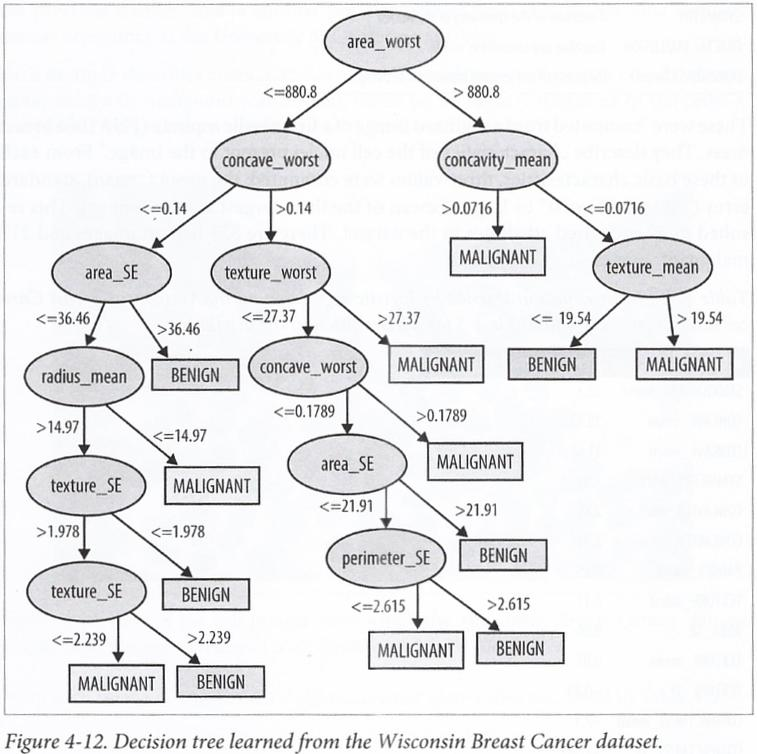
\includegraphics[width=0.5\textwidth]{4-12c_classification_tree.jpg}} \\
  \multirow{2}{*}{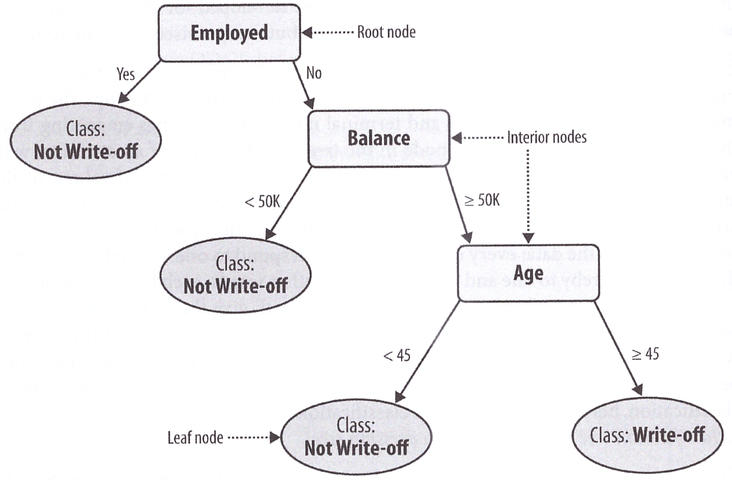
\includegraphics[width=0.5\textwidth]{3-10c_classification_tree.jpg}} & \\
  & {\vspace{14.5ex}\fontsize{10}{0}\selectfont \textbf{Source: [DSB]}} \\
  {\vspace{3ex}\fontsize{10}{10}\selectfont \textbf{Source: [DSB]}}&\multirow{2}{0.5\textwidth}{\tiny \emph{The picture above shows a classification tree for a real dataset relating to breast tissue scans examined for cancer. The target variable has values \textbf{MALIGNANT} and \textbf{BENIGN}. The attributes are numeric, categorized into ranges that produce a good predictive model.}} \\
\end{tabular}}
\newpage


{\setstretch{0.8}
\begin{tabular}{p{0.45\textwidth}p{0.4\textwidth}}
  \multirow{3}{*}{\vspace{-10ex}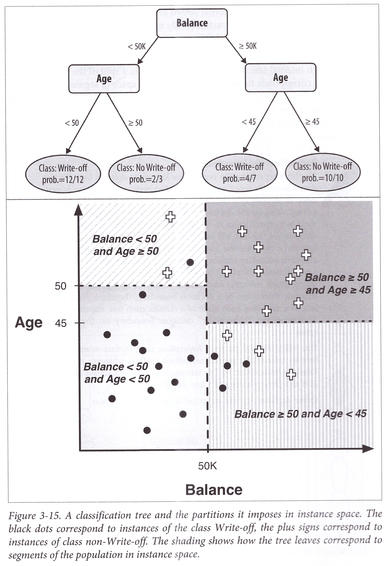
\includegraphics[width=0.45\textwidth]{3-15c_classification_space.jpg}} & \\ 
  & {\vspace{10ex}\headerss{Segment visualization}} \\
  & {\tiny \emph{The picture shows a classification tree using two attributes: \textbf{Balance} and \textbf{Age}. With two attributes, it is possible to show the data in a two dimensional co-ordinate system, together with the lines along which the data set is split. The splitting for this particular set could be improved, for example if the age categorization boundary were changed to 55 for Balance $<$ 50K, the two data subsets for Balance $<$ 50K would be pure.}\vspace{19ex}} \\ 
  {\fontsize{10}{0}\selectfont \textbf{Source: [DSB]}} & \\
\end{tabular}}
\newpage

% ----------------------------------------------------------------
% PAGE REGRESSION TREES
% ----------------------------------------------------------------
\headerch{Regression trees}
\hypertargettopofpage{regression-trees}
\begin{itemize}
\item Regression trees are built for \emph{continuous numeric target variables}
\item Predictions made by a regression tree model are in the form of a numeric value  
\item Instead of measures of impurity, regression tree building algorithms use \emph{variance} to define splitting criteria
\item Variance is used in the context of a test such as ANOVA, which evaluates splits based on variance within and between subsets: the most informative split is that with the greatest difference between inter-subset and intra-subset variance
\end{itemize}
\cornertab{N H N N N N N N F F F F F F}
\vfill
\newpage

% ----------------------------------------------------------------
% PAGE PROBABILITY ESTIMATION
% ----------------------------------------------------------------
\headerch{Probability estimation trees}
\hypertargettopofpage{probability-estimation-trees}
\cornertab{N N H N N N N N F F F F F F}
\begin{itemize}
\item Apart from classification and regression, tree models can be used to determine the \emph{probability} of a data instance belonging to a certain class
\item There are many applications for which probability estimation is the more appropriate approach than classification:
  \begin{itemize}
  \item Identification of segments with highest probability of class membership in situations where the overall probability is very low. For example, if a bank is trying to identify the customers that are likely to default on their mortgage and the probability of default is low in all segments of the customer population, a classification model would classify all the segments as \textbf{not likely to default} and would not be very useful. A probability estimation model would distinguish between probabilities in the different segments, e.g. 0.5, 0.3 and 0.1, all low but different!
  \item Ranking of data instances by probability. For example, if a company has a budget to spend on customer retention, they may want to rank all the customers by probability of leaving and offer incentives to the number of highest ranking potential leavers that the budget allows.
  \item \emph{Probability estimation trees} are induced using the same principles as classification trees
  \item Probability of class membership for a segment (corresponding to a leaf data subset in a tree), is estimated using the following formula:
    $$p(c) = \dfrac{n+1}{n+m+2}$$
    where $c$ is the class, $n$ is the number of instances belonging to class $c$ and $m$ is the number of instances not belonging to class $c$. The formula $p(c)=n/(m+n)$ intuitively seems more appropriate, however, the \emph{Laplace correction} is included to account for effects of small data subsets. 
  \end{itemize}
\end{itemize}

\newpage


{\setstretch{0.8}
\begin{tabular}{p{0.44\textwidth}p{0.44\textwidth}}
  \headerss{Examples} & \\
  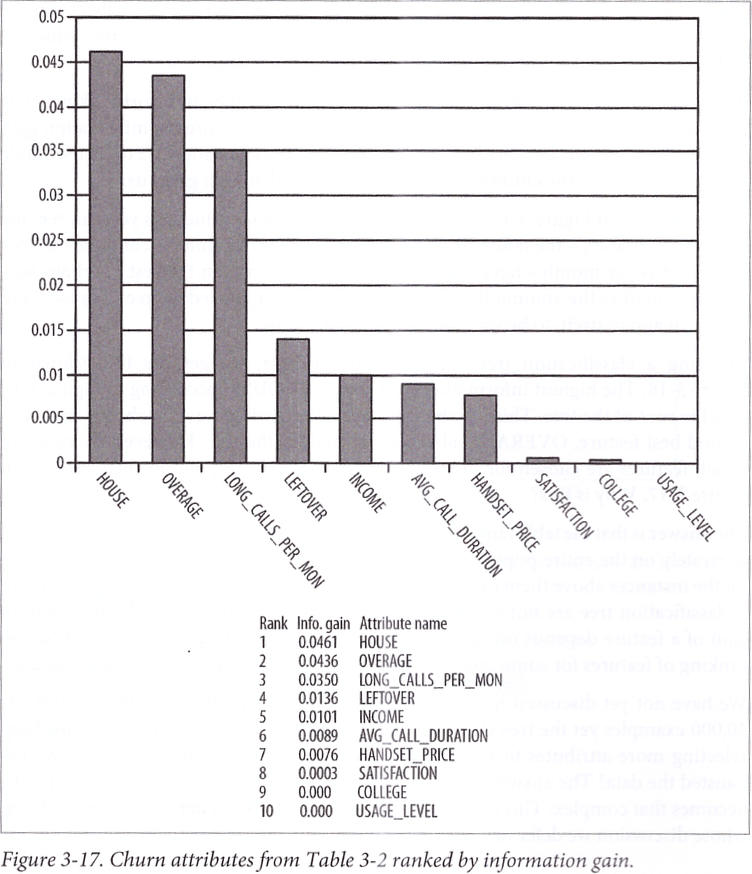
\includegraphics[width=0.44\textwidth]{3-17c_prob_est_tree_attribs.jpg} &
  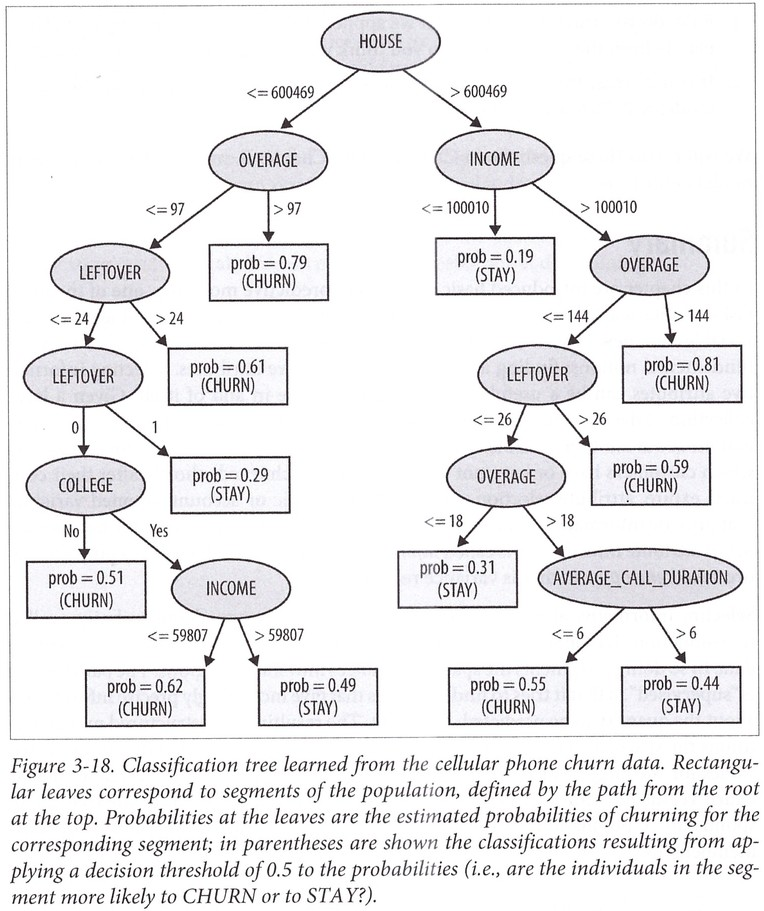
\includegraphics[width=0.44\textwidth]{3-18c_prob_est_tree.jpg} \\ [-1.5ex]
{\fontsize{10}{0}\selectfont \textbf{Source: [DSB]}} & 
{\fontsize{10}{0}\selectfont \textbf{Source: [DSB]}} \\
\multicolumn{2}{p{0.9\textwidth}}{\tiny \emph{A probability estimation tree for target variable with values \textbf{CHURN} and \textbf{STAY}, regarding the likelyhood of the customers of a mobile phone company to leave. The picture on the left lists the attributes that are used in the tree shown in the picture on the right.}} \\ 
\end{tabular}}
\newpage


% ----------------------------------------------------------------
% PAGE LINEAR CLASSIFIERS
% ----------------------------------------------------------------
\headerch{Linear classifiers}
\hypertargettopofpage{linear-classifiers}
\begin{itemize}
\item A linear classifier as a predictive model has numeric inputs and a categorical value as output
\item A linear classifier is most easily illustrated in a two-dimensional cartesian coordinate system, where data instances labelled by the value of the categorical target variable are shown at the points defined by their attribute values. The linear classifier is a straight line that splits the entire space into two parts, each containing as homogeneous as possible a data subset with regard to the target variable (see examples below).
\item This idea can be extended to any number of dimensions, corresponding to the same number of attributes, with the dividing artefact being an $(n-1)$-dimensional plane, where $n$ is the number of attributes.
\item The form of the general linear model is:
  $$ f(x) = w_0 + w_1 x_1 + w_2 x_2 ... + w_{n-1} x_{n-1} $$
  where $n$ is the number of variables, $x_i$ are the attributes and $w_i$ are the linear function parameters. The function $f(x)$ is called the \emph{linear discriminant function}.
\cornertab{N N N H H H N N F F F F F F}

\item The aim of linear classification is to find the geometrical artefact that best divides the attribute space with respect to the target classes (target variable values). This line, plane or hyperplane (the term used for a plane with more than 2 dimensions) is expressed as
  $$f(x) = 0$$
  and its parameters parameters (weights) $w_i$ are chosen by a process of optimization, or learning, with an exact objective that depends on the method used.
  \item Once the weights are determined i.e. learned, the linear discriminant function can be used to assign new data instances to classes, with $f(x)>0$ placing data instance $x$ in one class and $f(x)\leq0$ in the other. 
  \item The weights, $w_i$, can be interpreted as a measure of importance of the attibutes to which they apply, provided the attribute values were normalised preceding the weight learning (optimization) process.
  \item The most common linear classifier methods  are:
  \begin{itemize}
  \item Logistic regression
  \item Support Vector Machines
  \end{itemize}
\end{itemize}
\newpage

\begin{tabular}{p{0.4\textwidth}p{0.4\textwidth}}
  \headerss{Examples} & \\
  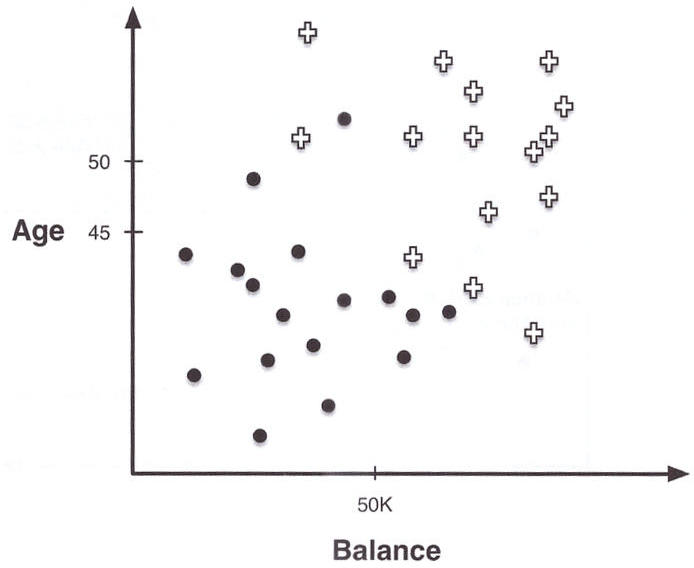
\includegraphics[width=0.4\textwidth]{4-2cc_two_attrib_space.jpg}&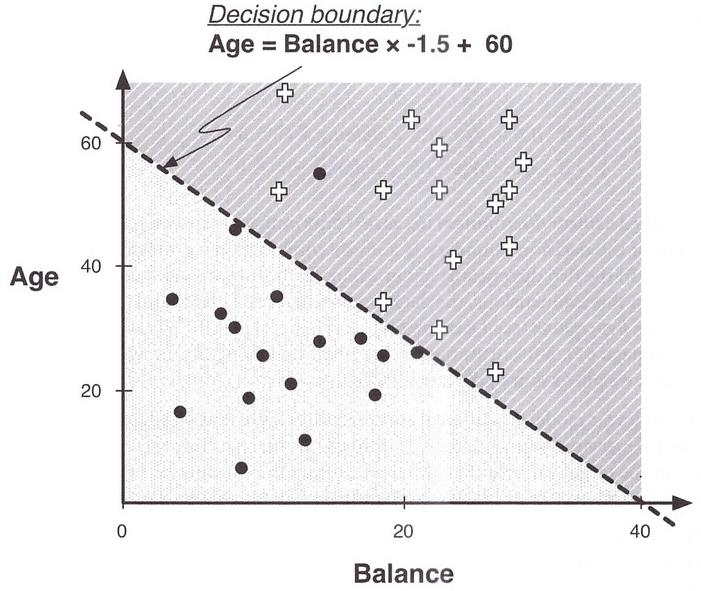
\includegraphics[width=0.4\textwidth]{4-3cc_general_linear_classifier.jpg} \\ [-1.5ex]
{\fontsize{10}{0}\selectfont \textbf{Source: [DSB]}} & 
{\fontsize{10}{0}\selectfont \textbf{Source: [DSB]}} \\
  \multicolumn{2}{p{0.8\textwidth}}{\tiny \emph{The picture on the left shows the same data set as that shown for segment visualisation, but without the splitting lines. A boundary line is shown alongside its linear formula using attributes \textbf{Balannce} and \textbf{Age}.}} \\
\end{tabular}
\newpage

\begin{tabular}{p{0.45\textwidth}p{0.45\textwidth}}
  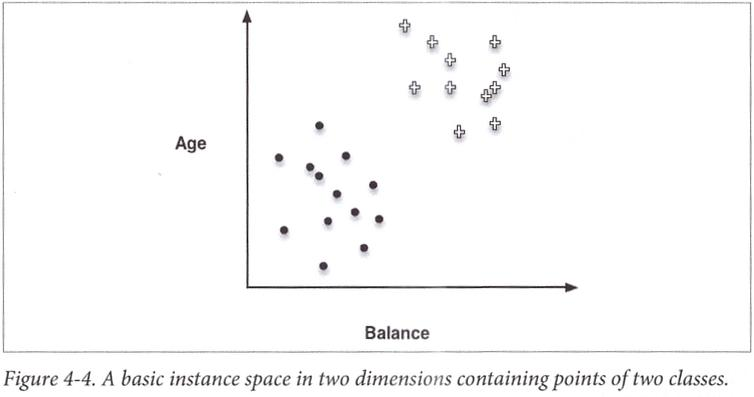
\includegraphics[width=0.45\textwidth]{4-4c_two_attrib_space.jpg}&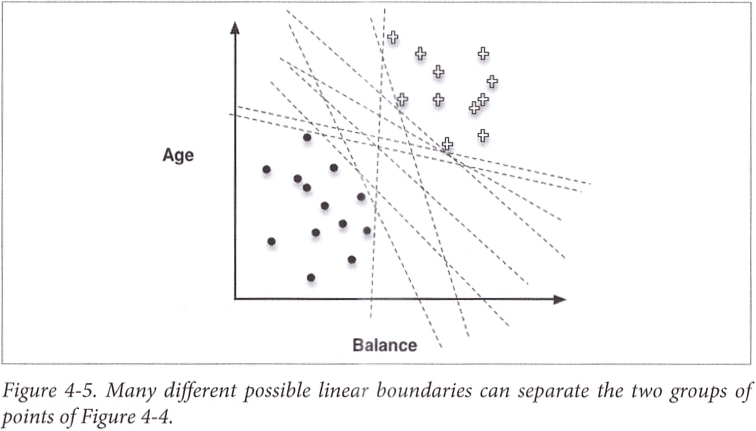
\includegraphics[width=0.45\textwidth]{4-5c_general_linear_classifier.jpg} \\ [-1.5ex]
{\fontsize{10}{0}\selectfont \textbf{Source: [DSB]}} & 
{\fontsize{10}{0}\selectfont \textbf{Source: [DSB]}} \\
  \multicolumn{2}{p{0.9\textwidth}}{\tiny \emph{The picture on the left shows another dataset in the two-attribute space, while the one on the right illustrates a few of the infinite number of ways in which the linear discriminant could be defined.}} \\
\end{tabular}
\newpage

% ----------------------------------------------------------------
% PAGE LOGISTIC REGRESSION
% ----------------------------------------------------------------
\headerch{Logistic regression}
\hypertargettopofpage{logistic-regression}
\begin{itemize}
\item Logistic regression is, in spite of its name, in fact a classification model. Its input attibutes are numerical and the output is either a category or a probability of belonging to a category.
{\hspace*{-3ex}
  \begin{tabular}{p{0.35\textwidth}p{0.6\textwidth}}
    \vspace{0ex}
   \multirow{1}{0.35\textwidth}{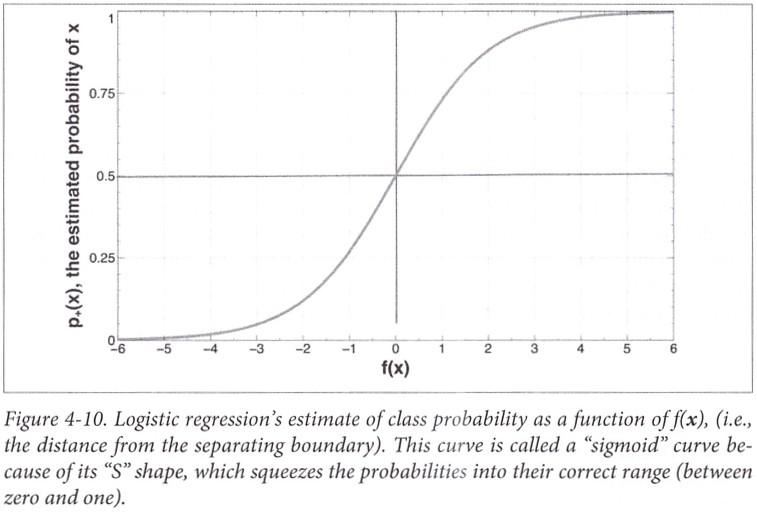
\includegraphics[width=0.35\textwidth]{4-10c_log_reg_sig.jpg}} & \multirow{1}{0.6\textwidth}{\vspace{-2ex}\begin{itemize}
      \renewcommand{\labelitemii}{$\bullet$}
      \item Instead of using the linear discriminant function, it uses a transformation of it:
        $$p_{+}(x) = \dfrac{1}{1+e^{-f(x)}}$$
        where $p_{+}(x)$ is the probability of data instance x belonging to a particular class (having one of two target variable values), $f(x)$ and is a function identical to the linear discriminant function.
      \end{itemize}} \\ [18.5ex]
 {\fontsize{10}{0}\selectfont \textbf{Source: [DSB]}} & \\
  \end{tabular}}
  \item The value of $p_{+}(x)$ is limited to the range between $-1.0$ and $1.0$ and once the model is in place (i.e. the parameter values have been learned) and given a new data instance, the logistic model outputs a probability of the instance belonging to the class of interest
  \item Defining a probability threshold (e.g. 0.5), allows the use of the logistic model for classification.
\cornertab{N N N N H N N N F F F F F F}
\end{itemize}
\newpage


% ----------------------------------------------------------------
% PAGE SUPPORT VECTOR MACHINES
% ----------------------------------------------------------------
\headerch{Support Vector Machines}
\hypertargettopofpage{svm}
\begin{itemize}
\item Support Vector Machines are another type of linear classifier. \\
{\hspace*{-4ex}
  \begin{tabular}{p{0.35\textwidth}p{0.45\textwidth}}
    \vspace{0ex}
   \multirow{1}{0.35\textwidth}{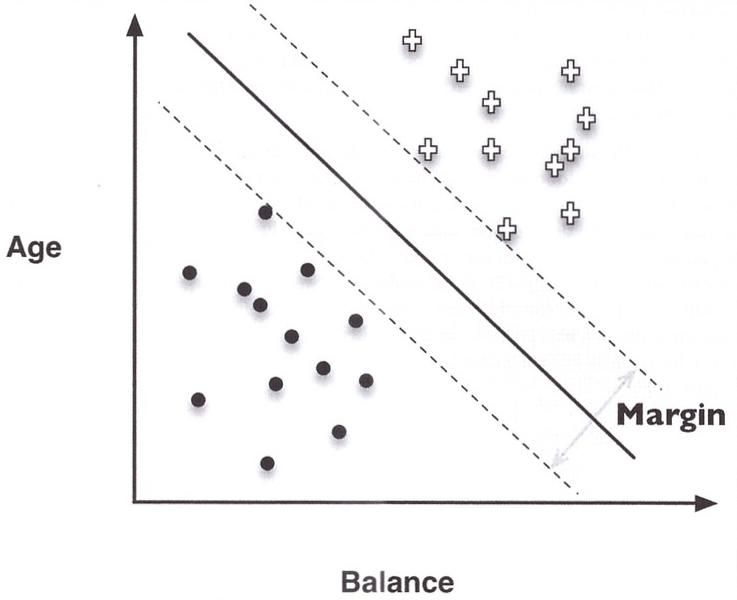
\includegraphics[width=0.35\textwidth]{4-8cc_SVM.jpg}} & \multirow{1}{0.45\textwidth}{\vspace{-1ex}\begin{itemize}
      \renewcommand{\labelitemii}{$\bullet$}
      \item The boundary line (or plane or hyperplane) is determined by finding the maximal margin that can be achieved between data instances, with respect to attribute values, between instances belonging to one target class and those belonging to the other. The boundary is drawn along the middle of the margin-wide strip. 
      \end{itemize}} \\ [23ex]
 {\fontsize{10}{0}\selectfont \textbf{Source: [DSB]}} & \\
    \multicolumn{2}{p{0.8\textwidth}}{\begin{itemize}[leftmargin=2ex]
     \renewcommand{\labelitemii}{$\bullet$}
     \item If the data instances cannot be cleanly separated in this manner, a margin-wide strip is still defined, with the optimization including 'penalties' to account for data instances 'on the wrong side' of the boundary 
      \end{itemize}} 
  \end{tabular}}
\cornertab{N N N N N H N N F F F F F F}
\end{itemize}
\newpage


% ----------------------------------------------------------------
% PAGE NON-LINEAR CLASSIFIERS
% ----------------------------------------------------------------
\headerch{Non-linear classifiers} 
\hypertargettopofpage{non-linear-classifiers}

Classification methods may use non-linear functions (where the attribute values contribute with a power other than 1). In this case the boundary line for classification is not straight. \\
  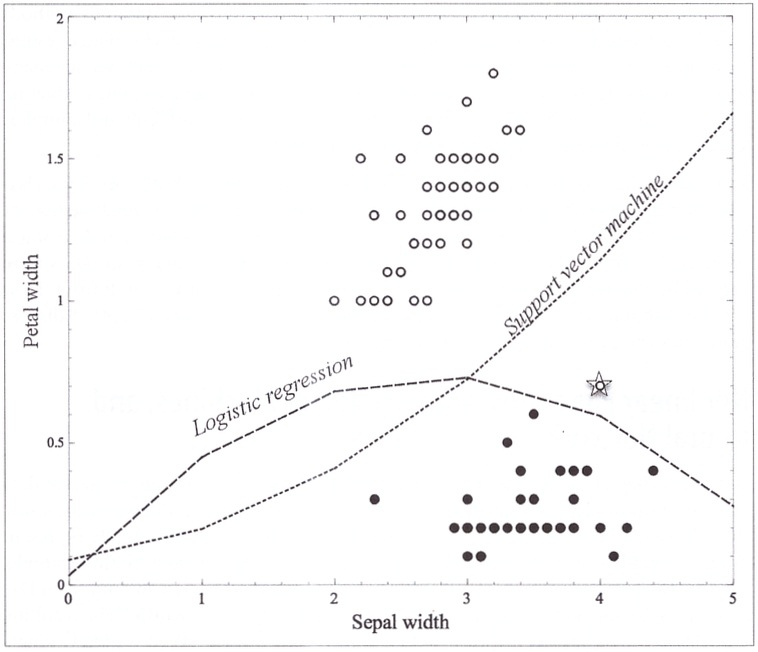
\includegraphics[width=0.4\textwidth]{4-13cc_non-linear_classifiers.jpg} \parbox[t]{0.3\textwidth}{\vspace{-20ex}\tiny \emph{The picture shows data being classified using non-linear logistic regression and a non-linear support vectory machine. }} \\ [-2ex]
  {\fontsize{10}{0}\selectfont \textbf{Source: [MSD]}} 
  \cornertab{N N N N N N H N F F F F F F}
\newpage
  
%----------------------------------------------------------------
% PAGE REGRESSION
% ----------------------------------------------------------------
\headerch{Statistical regression}
\hypertargettopofpage{regression}
\begin{itemize}
\item Statistical regression models can be linear and non-linear, single variable and multi-variate.
\item As a prediction model, regression takes numeric inputs and produces numeric outputs.
\item A regression model is \emph{fitted} using known data, then used for the prediction of the dependent variable in data where it is not known. 
\item We will be looking at linear regression only, but the principles can be extended to the other types of regression.
\item A linear regression model can be generated if there is a linear relationship between the independent and dependent variable.
\item The mathematical model for linear regression is the same linear function as used for classification:
\cornertab{N N N N N N N H F F F F F F}
    $$ f(x) = w_0 + w_1 x_1 + w_2 x_2 ... + w_{n-1} x_{n-1} $$
    where $x_1$, $x_2$...$ x_n$ are the independent variables and $w_0$, $w_1$, $w_2$... $w_n$ are the coefficients of the linear function. With regression, $f(x)$ corresponds to the dependent variable and the coefficients are chosen on the principle of minimizing the average distance of the existing data observations from the model line (or plane or hyperplane). The model \emph{represents the relationship} between the independent variables on one side and the dependent variable on the other: given a new observation, the dependent variable can be deduced from the independent variables by using the model. In the case of classification the purpose of the line was to \emph{divide the space} and hence define subsets of the data.
\end{itemize}
  
\headerss{Fitting a linear regression model}
\begin{itemize}
\item A linear regression model with one independent variable can be fitted 'manually'.\\ [1ex]
  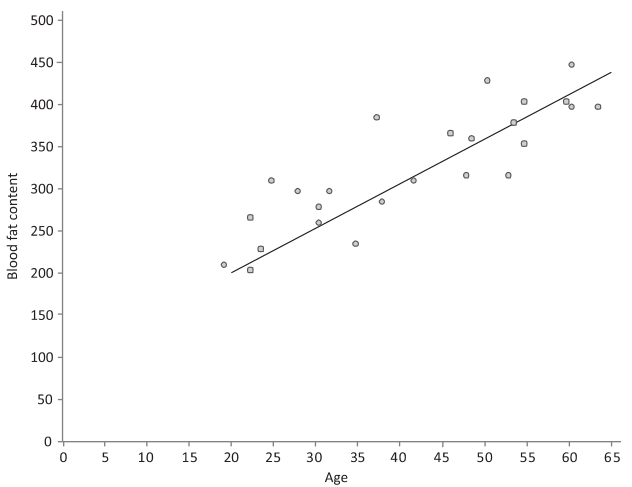
\includegraphics[width=0.3\textwidth]{msd6-5_linear_regression.png} \parbox[t]{0.3\textwidth}{\vspace{-20ex}\tiny \emph{The picture shows an example of some data with one independent variable together with the fitted regression line.}} \\ [-2ex]
  {\fontsize{10}{0}\selectfont \textbf{Source: [MSD]}} 
\item The regression line formula is:
  $$ y = a + bx$$
  where y is the dependent variable, x is the independent variable and $a$ and $b$ are the coefficients of the linear function.
\item The coefficient $b$, which is in face the slope of the line, is calculated as follows:
  $$ b = \dfrac{\mathlarger{\mathlarger{\sum}}_{i=1}^n(x_i-\mean{x})(y_i-\mean{y})}{\mathlarger{\mathlarger{\sum}}_{i=1}^n(x_i-\mean{x})^2} $$
  where $x_i$ and $y_i$ are the independent and dependent variable values for the $i^{th}$ observation, $n$ is the number of observations and $\mean{x}$ and $\mean{y}$ are the means of the independent and dependent variable, respectively. \\
\item The coefficient $a$ can be calculated by substituting the variables in the equasion by the means:
  $$ a = \mean{y} - b\times \mean{x} $$
\item Fitting a model with more than one independent variable is more complicated and is generally done using a computer.
\end{itemize}
\newpage


% ----------------------------------------------------------------
% PAGE K-NN
% ----------------------------------------------------------------
\headerch{k-Nearest Neighbours (k-NN)}
\begin{itemize}
\item This method can be used with any types of attributes and target variables
\item It is an \textbf{algorithm} for determining a target variable's value for a data instance, given a labelled data set (one in which the target variable's value is known for all instances)
\end{itemize}
\vspace{3ex}
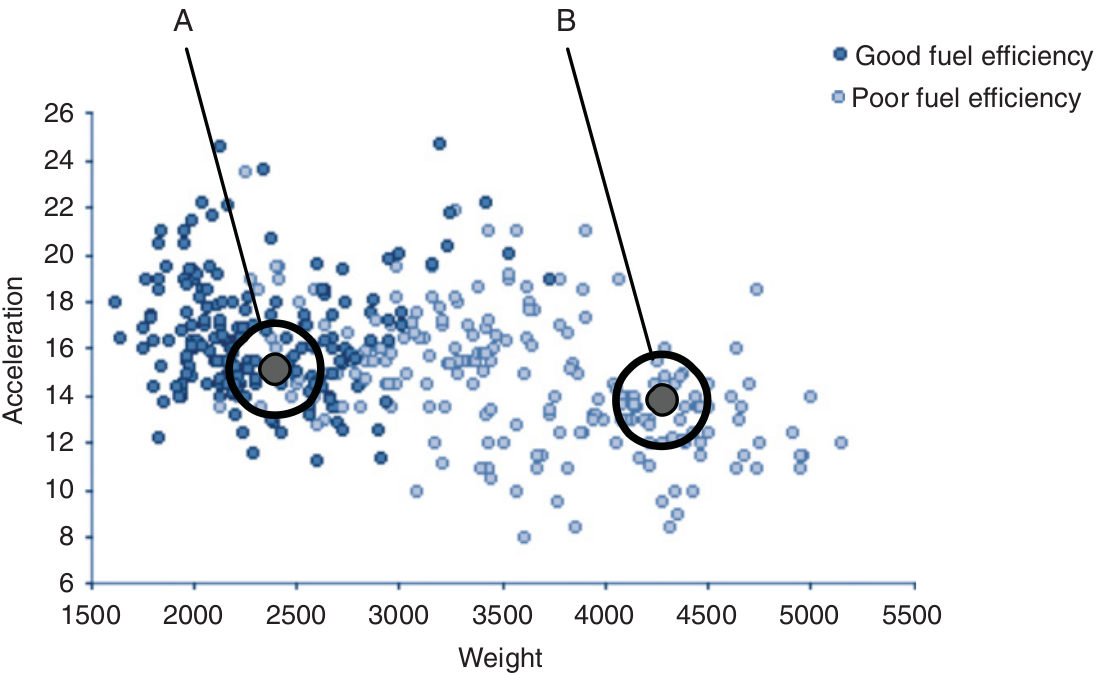
\includegraphics[width=0.4\textwidth]{msd6-13_k_nearest_neighbours.png}\parbox[t]{0.6\textwidth}{\vspace{-20ex}
\begin{itemize}
\item The distance is calculated between the new data instance and the instances in the dataset, based on the values of the attributes, which can be numeric (distance is Euclidean) or categorical (some measure of distance e.g. Jaccard)
\item The target variable of the new instance is calculated based on the target variable values of the closest $k$ instances (e.g. as average if numeric or most frequent value if categorical)
\item Determining the best value for $k$ is also part of the algorithm
\end{itemize}
} \\ [-12.5ex]
{\fontsize{10}{10}\selectfont \textbf{Source: [MSD]}}\\
\parbox[t]{0.4\textwidth}{\tiny \emph{In the picture \textbf{fuel efficiency} (possible values: \textbf{Good} and \textbf{Bad}) is determined for two cars, based on existing fuel efficiency data as related to weight and acceleration, using k-NN.}}
  \cornertab{N N N N N N N N H H H H H H}
\newpage

% ----------------------------------------------------------------
% PAGE NEURAL NETWORKS
% ----------------------------------------------------------------
\vspace*{1ex}
\headerch{Artificial neural networks (ANN)}
\begin{itemize}
\item Computational models that loosely emulate the workings of a brain
\item ANNs can be designed for any kind of input and output variable types
\item They are non-linear models, with parameters (weights) that need to be fitted to data
\item The structure of an ANN consists of nodes and connections between those nodes:
  \begin{itemize}
  \item a node applies a weight to the value that enters it, despatching the new value further into the network
  \item the connections define the flow of information between nodes
  \item the input attributes are 'fed' into the first layer of nodes and the output values received from the last layer
  \end{itemize}
  \item The learning, i.e. parameter fitting, in an ANN takes place through multiple cycles of data flowing through the network and weight adjustments using a suitable algorithm 
\end{itemize}
\cornertab{N N N N N N N N H H H H H H}
\newpage

% ----------------------------------------------------------------
% PAGE Overfitting
% ----------------------------------------------------------------
\headerch{Overfitting}
\begin{itemize}
\item \emph{Overfitting} is the application of model-building procedures to an extent that causes the created model to include properties specific to the training data, in addition to those actually pertinent to a general model
\item For example:
  \begin{itemize}
  \item a classification tree can be refined until all the leaf nodes are pure, but in most cases such a tree is over-fitted
  \item with a mathematical function overfitting may occur through the addition of too many attributes: more attributes means more dimensions and a better fit, but to the detriment of general applicability
  \end{itemize}
\item Overfitting can be avoided by using \emph{holdout} data to test that the accurracy of a model when used on new data matches, or is close to, the accuracy of the model when used on training data
\end{itemize}
\newpage

{\setstretch{0.8}
  \begin{tabular}{p{0.5\textwidth}p{0.5\textwidth}}
    \headerss{Examples}& \\
    \multicolumn{2}{p{0.9\textwidth}}{\tiny \emph{The optimal complexity of a particular type of model built with some data set can be determined with the help of a \textbf{fitting graph}. A fitting graph plots the accuracy of models of increasing complexity (e.g. represented by the number of nodes if a model is a decision tree), both for the training set and for a test set. As the complexity increases, so does the accuracy for both the training and test (holdout) set, until a critical complexity value at which the accuracy for the two sets diverges. It is for complexity higher than this critical value that the model is overfitted.}} \\
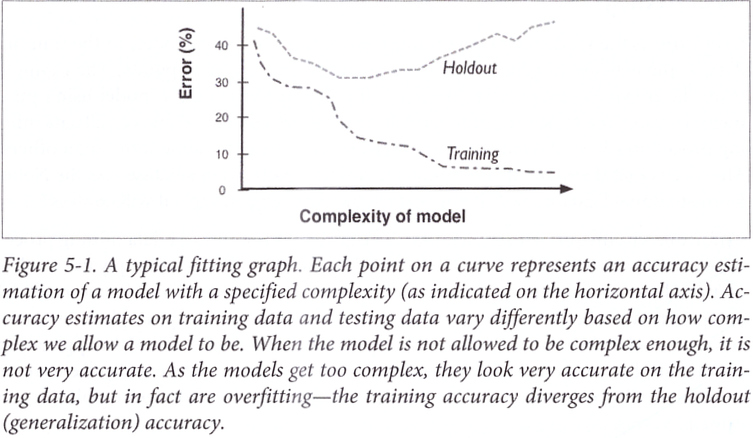
\includegraphics[width=0.5\textwidth]{5-1c_overfitting.jpg} &
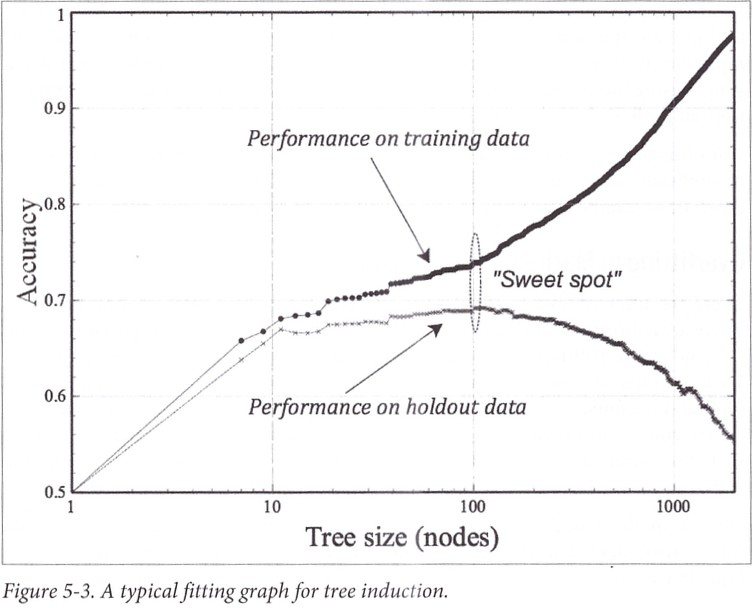
\includegraphics[width=0.4\textwidth]{5-3c_tree_overfitting.jpg} \\ [-1.5ex]
{\fontsize{10}{0}\selectfont \textbf{Source: [DSB]}}& {\fontsize{10}{0}\selectfont \textbf{Source: [DSB]}} \\
\end{tabular}}


\newpage

%----------------------------------------------------------------
% PAGE MODEL EVALUATION
% ----------------------------------------------------------------
% \headerch{Model evaluation}
% Moved into separate file "Model Performance"


%----------------------------------------------------------------
% PAGE REFERENCES
% ----------------------------------------------------------------
\headersec{References}

The pictures in this presentation were taken from the following books. The source for each picture is cited beside it. 

\textbf{[DSB]} \emph{Data Science for Business: What you need to know about data mining and data-analytic thinking}, by Foster Provost and Tom Fawcett, O'Reilly Media, 2013. 

\textbf{[MSD]} \emph{Making Sense of Data I: A Practical Guide to Exploratory Data Analysis and Data Mining}, by Glenn J. Myatt and Wayne P. Johnson, John Wiley \& Sons, 2014. 





\end{document}


